% =========================
\appendix


%%%%%%%%%%%%%%%%%%%%%%%%
\chapter{Density estimation: mathematical derivations}
\label{apx:DEMath}
\section{Embedding time series with Gaussian processes hyperparameters}
\label{apx:GPEmbed}
A Gaussian process (GP) \cite{rasmussen2006cki} is \emph{a collection of random variables, any finite number of which have a joint Gaussian distribution}.

A Gaussian process $f(x)$ is fully specified by a mean function $\mu(x)$ and a covariance function, or a kernel, $k(x,x')$, by-way-of:

\begin{align}
    m(x) &= \E[f(x)] \\
k(x,x') &= \E[(f(x)-m(x))(f(x')-m(x')]
\end{align}

And it is denoted:

\begin{align}
    f(x) \sim \mathcal{GP}(m(x), k(x,x'))
\end{align}

In this work we will take the mean function to be zero.

\subsubsection{parameter estimation (inference)}
Gaussian processes are commonly used for time series modeling with machine learning. To see why this makes sense, imagine the input $x$ is the time point, and the output $f(x)$ is the time series value at time $x$. Computationally, this is made feasible by evaluating the function's values at a finite number of points of interest.
Using optimization techniques, the model's hyperparameters are inferred to match observed data by maximizing the likelihood function $p(f(x) \mid \Vec{\theta})$ (termed maximum likelihood estimation, or MLE). The learned hyperparameters capture global evolutionary dynamics of the time series.

%  (see figure \ref{fig:3methods:posterior_draws} in the Methods section)

\subsubsection{The Matérn class of covariance functions}
The Matérn class of covariance functions is given by:

\begin{align}
    k_{Matern}(x,x') = \frac{2^{(1-\nu)}}{\Gamma(\nu)}(\sqrt{2\nu}d)^\nu K_\nu (\sqrt{2\nu}d)
\end{align}

Where:
\begin{itemize}
    \item $d = (x-x')^T \Phi^{-2} (x - x')$ is the distance between $x$ and $x'$ scaled by the \emph{lengthscale} parameter $\Phi$.
    \item $\nu$ is a smoothness parameter. In this work, it is taken to be $\frac{3}{2}$.
    \item $K_\nu$ is a modified Bessel function.
\end{itemize}

\subsubsection{Multitask Gaussian processes}
In case $f(x)$ is a vector function, multiple output functions are modeled in conjunction for the same input values, so-called multitask Gaussian process modeling. In this case, given inputs $x$ and $x'$, and tasks $i$ and $j$, the covariance between two datapoints and two tasks is given by:

\begin{align}
\label{eq:2background:multitask}
    k([x,i], [x',j]) = k_{inputs}(x,x') \cdot k_{tasks}(i,j)
\end{align}

Where $k_{inputs}$ is a standard kernel (e.g., Matérn) that operates on the inputs, and $k_{tasks}$ is a lookup table containing inter-task covariance. This is akin to capturing the inter-channel synchronicity with manually engineered features (see section \ref{sec:c2:features}).


\subsubsection{Gaussian process parameters embedding}
Inference of Gaussian process (GP) parameters is a well-documented approach to modeling time-series data \cite{rasmussen2003gaussian}. The extension to multitask GPs enables modeling of multivariate time-series, such as the case of multi-lead EEG signals.

% \begin{figure}[htbp]
    \centering
    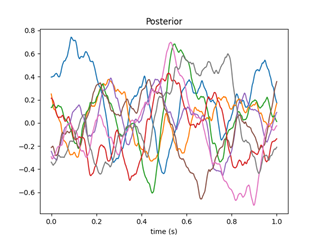
\includegraphics[width=0.4\floatwidth]{3Methods/Figs/GP/posterior_draws.png}
    \Caption{Embedding EEG with GP hyperparameters}{
	Posterior draws from a Gaussian process fit to maximize the likelihood of an observed single-channel EEG segment.
	\protect \NS[inline]{replace with vectorized image}
	\protect \NS[inline]{add original sample}
    }
    \label{fig:3methods:posterior_draws}
\end{figure}


For each EEG segment $x$, the preprocessing steps include:

\begin{enumerate}[label=\roman*]
    \item Normalizing $x$ by subtracting the mean and dividing by the standard deviation of the training set.
    \item initializing a GP model with zero mean, a scaled Matérn-1.5 kernel, and a rank-1 multitask covariance kernel.
    \item Optimizing the model's parameters to obtain a maximal marginal log-likelihood (details in appx. \ref{apx:GPTraining}).
\end{enumerate}

The optimized model's parameters $\theta$ are persisted and used henceforth to represent the original EEG segment $x$.


\section{Gaussian Mixture Models}
\label{apx:GMM}
Gaussian mixture models \cite{theodoridis2015machine} are used to model the distribution of an unknown set of vectors $\{x\} \subseteq \mathbb{R}^l$ as a linear combination (i.e., a mixture) of different Gaussian distributions, that is,

\begin{align}
    p(x) = \sum_{k=1}^{K}p_kp(x \mid k; \zeta_k)
\end{align}

where $\{\zeta_k\}$ parametrize the individual Gaussian distributions:
\begin{align}
    p(x \mid k ; \zeta_k) = p(x \mid k; \mu_k, \sigma_k) = \mathcal{N}(x \mid \mu_k, \sigma_k)
\end{align}

Fitting the model (e.g. via expectation maximization) provides an approximation $\hat p(x \mid k; \zeta_k)$ of the dataset's underlying pdf, which is an estimate of the data-distribution of the GP-hyperparameters $P(E \mid D)$


%%%%%%%%%%%%%%%%%
\chapter{GP embedding: training details}
\label{apx:GPTraining}

% =========================
For dimensionality reduction of an observed EEG segment, we performed exact inference of the GP parameters maximizing the observation likelihood, using the GPyTorch and PyTorch Lightning frameworks \shortcites{gardner2018gpytorch} \cite{gardner2018gpytorch, Falcon_PyTorch_Lightning_2019}.

More formally, in fitting the Gaussian processes to the EEG samples we carried out exact Type-II Maximum Likelihood Estimation for each sample. This means optimizing the model's hyperparameters (mean module, covariance module, etc.) w.r.t maximization of the \emph{marginal log likelihood} (MLL) of the given data $\mathbf{E, t}$:

\begin{align}
    \theta \gets \argmax_\theta p_f(\mathbf{E} \mid \mathbf{t}) = \int p(\mathbf{E} \mid f(\mathbf{t})) p(f(\mathbf{t}) \mid \mathbf{t}) df
\end{align}

where $f \sim \mathcal{GP}(\mu, K)$ is the modeled signal before adding the homescedastic Gaussian noise, and $\theta$ is the set of parameters to be optimized. See code for implementation details.

\begin{table}[h]
\begin{tabular}{ |p{3cm}||p{5cm}||p{5cm}| }
 \hline
 \multicolumn{3}{|c|}{GP \& inference (training) configuration details} \\
 \hline
  &Parameter& Value \\
 \hline
\multirow{5}{3cm}{GP params} & mean module & zero mean\\
&covariance module& scaled Matérn-1.5 kernel\\
&task covariance rank& 1 \\
&number of tasks& 2   \\
&likelihood (noise model)&Gaussian (homoscedastic)\\
\hline
\multirow{4}{3cm}{Training params}& optimizer &Adam\\
&learning rate& 0.01 \\
&max. number of epochs & 1000\\
&patience (early stopping)&8 \\
 \hline
\end{tabular}
\caption{The GP parameters and training parameters used in our experiments.}
\label{table:GPTraining}
\end{table}

